\section{Theorie}
\label{sec:Theorie}

% In knapper Form sind die physikalischen Grundlagen des Versuches, des Messverfahrens, sowie sämtliche für die Auswertung erforderlichen Gleichungen darzustellen. (Keine Herleitung)

% (eventuell die Aufgaben)

% Der Versuchsaufbau: Beschreibung des Versuchs und der Funktionsweise (mit Skizze/Bild/Foto)

Ein Lock-In-Verstärker wird verwendet um stark verrauschte Signale und Spannungen zu messen.
Zuvor werden die  sehr hohen und sehr niedrigen Frequenzen des Eingangssignals durch einen Bandpassfilter geschwächt beziehungsweise ganz entfernt.
Eine Referenzspannung $U_\text{ref}$, mit der Frequenz der Eingangspannung $U_\text{sig}$, wird mit der Eingangspannung multipliziert.
Dadurch wird das zu messende Signal zwischen dem Rauschen stärker hervorgehoben.
In \autoref{fig:bild1} ist das Prinzip dieser Mulitplikation verdeutlicht.

\begin{figure}
    \centering
    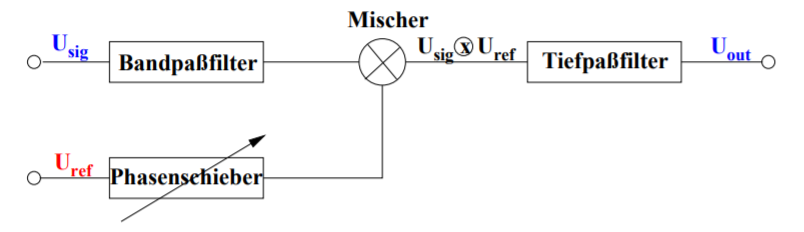
\includegraphics[width=\textwidth/2]{images/bild1.png}
    \caption{Funktionsweise eines Lock-In-Verstärkers.\cite{V303}}
    \label{fig:bild1}
\end{figure}

Bei einem einkommenden Signal 

\begin{equation}
    U_\text{sig} = U_0 \cdot \sin{\left(\omega \cdot t\right)}
    \label{eq:u_sig}
\end{equation}

und einer Rechteckspannung als Referenzspannung

\begin{equation}
    U_\text{ref} = \frac{4}{\pi} \left(\sin{\left(\omega \cdot t\right)} + \frac{1}{3}\sin{\left(3\omega \cdot t\right)} +  \frac{1}{5}\sin{\left(5\omega \cdot t\right)} + ...\right),
    \label{eq:u_ref}
\end{equation}

die durch eine Fourierreihe angenähert wird, ergibt sich für die Mulitplikation beider Signale 

\begin{equation}
    U_\text{sig} \times U_\text{ref} = \frac{2}{\pi} \cdot U_0 \left(1 - \frac{2}{3}\cos{\left(2\omega \cdot t\right)}  -  \frac{2}{15}\cos{\left(4\omega \cdot t\right)} - \frac{2}{35}\cos{\left(6\omega \cdot t\right)}...\right).
    \label{eq:u_ref_sig}
\end{equation}

$U_0$ ist dabei die Amplitude des Eingangssignals und $\omega$ die abgestimmte Frequenz der beiden Signale.
Das daraus entstehene Signal wird zuletzt durch einen Tiefpassfilter geschickt.
Dieser Tiefpassfilter besteht aus einer Kapazität $C$ und einem Widerstand $R$, diese sind über die Zeitkonstene $\tau$ verbunden und definierten zusammen die Bandbreite

\begin{equation}
    \Delta \nu = \frac{1}{\pi R \cdot C}
    \label{eq:tau}
\end{equation}

dieses Filters.
Dadurch filtern sich alle unerwünschten Anteile heraus und es bleibt nur eine Gleichspannung $U_\text{out}$ 

\begin{equation}
    U_\text{out} = \frac{2}{\pi} U_0 \cdot \cos{\left(\phi\right)}
    \label{eq:u_out}
\end{equation}

übrig.
Die Ausgangspannung ist proportional zur Eingangssignals und hängt von der Phasendifferenz $\phi$ ab. 